

\chapter{Serial Communication \label{seriali}} \hypertarget{def:seriali}{}

To use the simulator serial port, install a NULL-MODEM emulator:
\begin{itemize}
 \item Windows: com0com \url{http://sourceforge.net/projects/com0com/}
 \item Linux: tty0tty  \url{https://github.com/lcgamboa/tty0tty}
 \end{itemize}

For communication the PICSimLab should be connected in one port of the NULL-MODEM emulator and the other application connected in the other port.
Configuration examples linking PICSimLab to \href{https://github.com/neundorf/CuteCom}{Cutecom} for serial communication:
 \vspace{0.5cm}
 
 \begin{tabular}{|c|c|c|c|c|}
 \hline OS&  PicsimLab port&  Cutecom port & NULL-Modem prog. &Connection\\
 \hline 
 \hline Windows&  com1 & com2 &com0com &com1<=>com2\\
 \hline Linux &  /dev/tnt2 & /dev/tnt3 &tty0tty &/dev/tnt2<=>/dev/tnt3\\
 \hline 
 \end{tabular}
 
 \section{Com0com Installation and Configuration(Windows)}
 
 Download the signed version of \href{https://sourceforge.net/projects/com0com/files/com0com/3.0.0.0/com0com-3.0.0.0-i386-and-x64-signed.zip/download}{com0com}.
 
Unzip the downloaded .zip file and run the specific installer of your operating system, x86 for windows 32-bit or x64 for windows 64-bit.
 
Configure the ``choose components'' window as the figure below:
 \begin{figure}[H]
\center
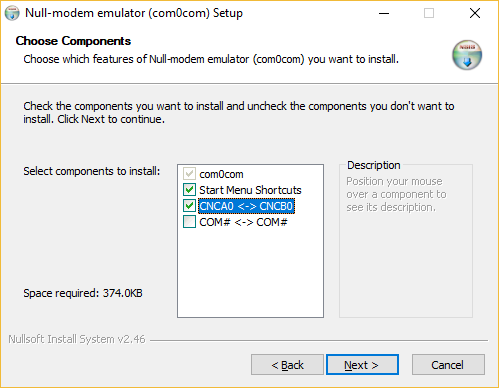
\includegraphics[width=0.8\textwidth]{img/com0com1.png} 
\end{figure} 


In the last configuration window, check the ``Launch setup'' option:
\begin{figure}[H]
\center
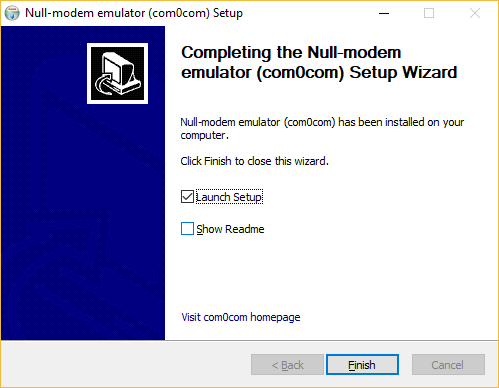
\includegraphics[width=0.8\textwidth]{img/com0com2.png} 
\end{figure} 

In the setup window, change the port names to COM1, COM2, COM3 ....
Just check the ``enable buffer overrun'' option on the two ports, click in the ``Apply'' button and close the setup.
In the configuration shown in the figure below, the COM1 and COM2 ports form a NULL-MODEM connection, where one port must be used by the PICSimLab and another by the application with serial communication.
\begin{figure}[H]
\center
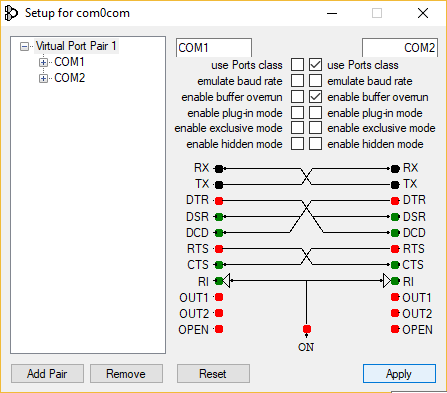
\includegraphics[width=0.8\textwidth]{img/com0com3.png} 
\end{figure} 
 
\section{tty0tty Installation and Configuration (Linux)}
 
Download the \ href {https://github.com/lcgamboa/tty0tty/archive/master.zip} {tty0tyy}.
Unzip the downloaded folder.
 
Open a terminal and enter in the tty0tty/module/ folder and enter the following commands:
\begin{verbatim}
 sudo apt-get update
 sudo apt-get -y upgrade
 sudo apt-get -y install gcc make linux-headers-`uname -r` 
 make
 sudo make install 
\end{verbatim}

The user must be in the \textbf{dialout} group to access the ports. 
To add your user to \textbf{dialout} group use the command:
\begin{verbatim}
sudo usermod -a -G dialout your_user_name
\end{verbatim}
after this is necessary logout and login to group permissions take effect.


Once installed, the module creates 8 interconnected ports as follows:
\begin{verbatim}
  /dev/tnt0  <=>  /dev/tnt1 
  /dev/tnt2  <=>  /dev/tnt3 
  /dev/tnt4  <=>  /dev/tnt5 
  /dev/tnt6  <=>  /dev/tnt7 
\end{verbatim}

the connection between each pair is of the form:
\begin{verbatim}  
  TX   ->  RX
  RX   <-  TX 	
  RTS  ->  CTS
  CTS  <-  RTS
  DSR  <-  DTR
  CD   <-  DTR
  DTR  ->  DSR
  DTR  ->  CD
\end{verbatim}

Any pair of ports form a NULL-MODEM connection, where one port must be used by the PICSimLab and another by the application with serial communication.
